\documentclass[12pt,a4paper]{jbook}
\usepackage{mm-thesis}
\usepackage[dvipdfmx]{graphicx}
\usepackage{cite}
\usepackage{comment}
\usepackage{docmute}
\usepackage{color}
\usepackage{moreverb}
\usepackage{listings}
\usepackage{ascmac}
%\usepackage{amsmath}
%\usepackage{amsthm}
%\usepackage{amsfonts}

\lstset{
	%枠外での自動改行
 	breaklines = true,
 	%標準の書体
 	basicstyle = {\small},
 	%枠 "t"は上に線を記載, "T"は上に二重線を記載
	%他オプション:leftline,topline,bottomline,lines,single,shadowbox
 	frame = TB,
 	%タブの大きさ
 	tabsize = 2,
 	%キャプションの場所("tb"ならば上下両方に記載)
 	captionpos = t,
 	%行番号の位置
 	numbers = left,
 	%自動改行後のインデント量(デフォルトでは20[pt])	
 	breakindent = 30pt,
	%左右の位置調整 	
 	xleftmargin=30pt,
 	xrightmargin=30pt,
	%プログラム言語(複数の言語に対応,C,C++も可)
 	%language = Python, 	
 	%背景色と透過度
 	%backgroundcolor={\color[gray]{.90}},
 	%コメントの書体
 	%commentstyle = {\itshape \color[cmyk]{1,0.4,1,0}},
 	%関数名等の色の設定
 	%classoffset = 0,
 	%キーワード(int, ifなど)の書体
 	%keywordstyle = {\bfseries \color[cmyk]{0,1,0,0}},
 	%表示する文字の書体
 	%stringstyle = {\ttfamily \color[rgb]{0,0,1}},
 	%frameまでの間隔(行番号とプログラムの間)
 	%framesep = 5pt,
 	%行番号の間隔
 	%stepnumber = 1,
	%行番号の書体
 	%numberstyle = \tiny,
}
\renewcommand{\lstlistingname}{Code}
\begin{document}

\chapter{既存のウェブセキュリティモデル}
この章では、セキュリティモデルの説明と、本研究の提案モデルの基礎となる既存のウェブセキュリティモデルについて説明する。

\section{セキュリティモデル}
\label{sec:SecurityModel}
セキュリティモデルは形式手法における入力にあたり、検査対象のシステムを命題論理を用いて表現したものである。
セキュリティモデルに記述する項目は主に以下の三つである。
\begin{itemize}
\item 対象のシステムの構造と動作
\item 脅威モデル(システムにとって脅威となりうるもののモデル 例:攻撃者の能力)
\item 安全性要件(システムが安全である場合に満たしているべき条件)
\end{itemize}

\section{今後の拡張を想定した基礎モデル}
\label{sec:based-model}

\subsection{モデルの特徴}
\label{sec:based-model-abstract}
Akhaweらによって提案されたウェブセキュリティモデル\cite{based-model}(以下、「基礎モデル」とする)は、後続するウェブの安全性解析に形式手法を用いることを意図して設計されたモデルである。
しかし、ウェブで運用されている要素の数は膨大であるため、現在の環境で頻繁に使用されている要素に注目して設計されている。

\subsection{基礎モデルの能力}
\label{sec:based-model-power}
基礎モデルが表現する内容を\ref{sec:SecurityModel}節の項目に従って説明する。

\subsubsection{対象のシステムの構造と動作}
ウェブには多様な要素が含まれており、それぞれの要素単体では安全が満たされていたとしても、組み合わせることで安全を侵害する動作が可能となることがある。
こういった危険な動作を引き起こすような複数の要素の関連を形式手法による安全性解析によって検出するため、まずは各要素のふるまいを明確に表現する必要がある。
ウェブセキュリティモデルにおいて、この項目にはそういった各要素のふるまいが含まれる。

\ref{sec:based-model-abstract}節で述べた通り基礎モデルは現在のウェブの環境において使用される頻度が高いものに限定して注目している。
以下にそれらの要素とそのふるまいを記述する。
\begin{itemize}
\item 非線形時間 \\
基礎モデルでは、時相論理として非線形時間軸を用いる。詳細は\ref{sec:based-model-temporal-logic}節に記述する。
\item ブラウザ \\
基礎モデルにおいて、ブラウザのモデルは大きく三つの観点から設計されている。

まず、ブラウザで動作するスクリプトについて述べる。
\color{red}
各スクリプトはある一つのオリジンに属する。
ここで、同様のオリジンに属するスクリプトは同様の権限を持つとする。
\color{black}
これは、異なるウェブページで動作していたとしても同じオリジンであれば、それらを一つのスクリプトとして取り扱うことを意味する。

次に、ブラウザ内のUIについて述べる。
ブラウザ内には、HTTPSにおけるグリーンバーのような、セキュリティに関する内容を示唆するUIが存在する。
このような安全性に関するUIは、基礎モデルで包括する。

最後に、メモリ領域について述べる。
基礎モデルでは、この領域をCookieやパスワードの保存領域として取り扱う。
この領域内の機密情報はある一つのオリジンとの関連を持ち、そのオリジンによるスクリプトによって読みだされる。
ただし、モデルの単純化のため、このメモリ領域は「追加」のみ可能とし、格納した情報の削除といった動作は包括しない。
\item サーバ \\
基礎モデルにおいて、サーバはIPアドレスで指定されるネットワーク上のある地点に存在するものとして取り扱う。
各サーバには一人の管理者が存在し、その管理者はそのサーバがリクエストに対してどう対応するかを制御することができる。
また、管理者が正当なユーザであればそのサーバは仕様に従った動作をするが、悪質なユーザ(攻撃者)であった場合はその限りではない。
また、サーバを指定するために用いられるDNSについても、基礎モデルでは取り扱う。
DNSは、例えば``www.example.com"というように、複数の名前で形成される階層構造を持つ。
こういった階層構造はDNS Rebinding\cite{dns-rebinding}といった攻撃を表現するために不可欠であるため、階層構造まで含めてモデルとして表現する。
\item ネットワーク \\
基礎モデルでは、ブラウザとサーバを接続するものとしてネットワークを取り扱う。
また、この項目は単純な通信経路を表すだけでなく、通信に用いられるプロトコルまで含めて表現する。
基礎モデルでの安全性解析で主に取り扱うHTTPについては詳細を\ref{sec:based-model-http}節で述べる。
このHTTPのモデルに加えて、リクエストやレスポンスにはそれを生成したAPIの種類によって異なる安全性要件が生じるため、これらを含めてモデルとして表現する。
\end{itemize}

\subsubsection{脅威モデル}
基礎モデルにおいて脅威モデルとして想定されている攻撃者の能力は三段階に分けられている。
この設計を利用し、どのレベルの攻撃者でどのような危険性が生じるのかといった、レベル毎の検査が可能である。

まず、三段階の脅威モデルのうち最も基本的なWeb Attackerの能力を以下に示す。
\begin{itemize}
\item ウェブサーバに対する能力 \\
Web Attackerは少なくとも一つのウェブサーバのroot権限を持ち、そのサーバへのリクエストに対して任意の内容でレスポンスを生成できる。
また、複数のDNSを所持し、それらのサーバに割り当てることができる。
これに加えて、正規の認証局から自身のドメインに対するサーバ証明書を取得することができる。
(例:Web Attackerはattacker.comというDNSを自身が運用するウェブサーバに割り当て、取得したサーバ証明書を用いてhttps://attacker.comへの接続を有効化できる)
\item 通信に対する能力 \\
Web Attackerは自信が運用するサーバへのリクエストに対するレスポンスの送信や、自身が所有する端末(クライアント)から正当なサーバに対してリクエストの送信のみができる。
このWeb Attackerが送信するリクエストはHTTPの仕様に従っている必要はない。
\item ウェブブラウザに対する能力 \\
あるブラウザがWeb Attackerのウェブサイトに一度でもアクセスした場合、Web AttackerはそのブラウザのAPIを自由に利用することができる。
ただし、攻撃者の使用するAPIはそのブラウザで設定されているセキュリティポリシーを超える動作を行うことはできない。
\end{itemize}

次に、Network Attackerは上記のWeb Attackerの全能力に加えて以下の能力を持つ。
\begin{itemize}
\item 暗号化されていない通信(例:HTTP通信)に対して、通信内容の傍受や改ざん、通信の遮断ができる
\item 基本的にHTTPSに対して介入することはできない。
しかし、正当な認証局から攻撃者の悪質なDNSに対してサーバ証明書を取得できている場合に限り、自己署名証明書を作成することができる。
つまり、この自己署名証明書を用いることで、HTTPS通信への傍受や介入が可能となる。
\end{itemize}

最後に、Gadget Attackerもまた、上記のWeb Attackerの全能力に加えて、正当なウェブサイトにいくつかの限定された形式の内容を挿入する能力を持つ。
この挿入できる内容の形式は使用されているウェブアプリケーションに依存し、多くの場合にハイパーリンクの挿入は可能である。

%edit:正当なユーザとは何か言及する
また、上記の攻撃者に加えて正当なユーザのふるまいに対しても制限が存在する。
これはユーザのふるまいを無制限とすることで、正当なユーザが攻撃者にパスワードを送信するといった安全性を侵す動作が検出されるなど、出力結果が膨大な数となることを防ぐためである。
しかし、逆にこの制限を強くしすぎると既出の典型的な攻撃法を見逃す恐れがあるため、程度の調整が重要である。
基礎モデルにおいては、これらのバランスを考慮し、正当なユーザふるまいに以下の制限が加えられている。
\begin{itemize}
\item ユーザは攻撃者のウェブサイトを含む複数のウェブサイトに接続することがある。
ただし、これにはユーザによる意図的な悪質なサイトへの接続は含まれない。
\item ユーザが攻撃者のサイトに接続したとしても、正当なサイトと混同することはない。
これは、ロケーションバーを始めとするブラウザのセキュリティ警告をユーザが正しく理解していることを前提とする。
\end{itemize}

\subsubsection{安全性要件}
基礎モデルでは、ウェブ全体の安全性要件として以下の二つの条件が定義されている。
\begin{itemize}
\item Security Invariants\\
ウェブ上の既存の各構成要素の仕様要件を侵さない。
つまり、各要素が仕様通りに動作していることが求められる。
\item Session Integrity\\
HTTPリクエストが正当なユーザによって生成されたものである。
なぜなら、HTTPサーバは受信したリクエストの内容に基づいて動作するため、そのリクエストが攻撃者によるものでないことを要求するためである。
\end{itemize}

\subsection{基礎モデルにおけるHTTPの実装}
\label{sec:based-model-http}

\subsubsection{リクエストとレスポンス}
基礎モデルにおいてリクエストとレスポンスはCode\ref{code:httpevent}のように表現される。
\begin{lstlisting}[caption=リクエストとレスポンスを表現するクラス, label=code:httpevent]
abstract sig Event {pre,post : Time}

abstract sig NetworkEvent extends Event {
	from: NetworkEndpoint,
	to: NetworkEndpoint
}

abstract sig HTTPEvent extends NetworkEvent {host : Origin}

sig HTTPRequest extends HTTPEvent { 
	method : Method,
	path : Path,
	queryString : set attributeNameValuePair,
	headers : set HTTPRequestHeader,
	body : set Token
}

sig HTTPResponse extends HTTPEvent {
	statusCode : Status,
	headers : set HTTPResponseHeader
}
\end{lstlisting}
コード内におけるextendsは継承関係を表し、例えば3行目においてはNetworkEventはEventを継承する。
まず、親クラスであるEventはウェブ上で発生するイベントを表し、Eventクラスに用意されているpre,postによって\ref{sec:based-model-temporal-logic}節で述べる時相論理の時間軸上で、そのイベントがどの時点で発生したかを表現できる。
次に、NetworkEventは
リクエストを表すHTTPRequestにはメソッド、ヘッダといった要素が含まれ、また、レスポンスを表すHTTPResponseには状態コード、ヘッダといった要素が含まれる。
基礎モデルの包括範囲では、リクエストとレスポンスのどちらにでも利用可能なヘッダを含めていないため、それぞれ別のエンティティで定義し混在することのないように記述している。

また、リクエストとレスポンスは対の対応関係があり、どのリクエストに対するレスポンスであるのかを明らかにできるよう、Code\ref{code:based-model-httptransaction}のようにHTTPTransactionクラスを作成している。
\begin{lstlisting}[caption=リクエストとレスポンスの対応関係, label=code:based-model-httptransaction]
sig HTTPTransaction {
	req : HTTPRequest,
	resp : lone HTTPResponse,
	cert : lone Certificate,
	cause : lone HTTPTransaction + RequestAPI
}{
	some resp implies {
		resp.host = req.host
		happensBeforeOrdering[req,resp]
	}

	req.host.schema = HTTPS implies some cert and some resp
	some cert implies req.host.schema = HTTPS
}
\end{lstlisting}
HTTPTransactionクラスはリクエストとそれに対応するレスポンスを保有する。
ただし、リクエストは必ずインスタンスが存在することに対し、レスポンスは一つ存在するか、もしくは存在しない場合がある。
これは何らかの要因でリクエストに応答がない場合があり、そういった場合には対応するレスポンスが存在しないことを表現している。
また、7-13行目ではHTTPTransactionが満たすべき条件が記述されており、特に9行目にはリクエストがレスポンスよりも前に発生しているという、時相論理を用いた条件が記述されている。

\subsubsection{ネットワークアプリケーション}
基礎モデルにおいて通信を行うネットワークアプリケーションはCode\ref{code:endpoint}のように表現される。
\begin{lstlisting}[caption=ネットワーク参加者, label=code:endpoint]
sig NetworkEndpoint{}

abstract sig HTTPConformist extends NetworkEndpoint{}

sig HTTPServer extends HTTPConformist{}

abstract sig HTTPClient extends HTTPConformist{
	owner:WebPrincipal
}

sig Browser extends HTTPClient {
	trustedCA : set certificateAuthority
}
\end{lstlisting}
親クラスであるNetworkEndpointはネットワーク上に存在するアプリケーションを表現するクラスである。
ただし、このクラスに含まれるアプリケーションはHTTPを遵守しているとは限らず、HTTPに遵守して動作するアプリケーションを表すクラスとしてHTTPConformistを定義している。
基礎モデルではHTTPを利用するアプリケーションとしてクライアントとサーバを包括しているため、このHTTPConformistを継承しHTTPClientとHTTPServerが定義されている。

\subsubsection{ネットワーク参加者}
基礎モデルにおいてリクエストとレスポンスはCode\ref{code:character}のように表現される。
\begin{lstlisting}[caption=ネットワーク参加者, label=code:character]
abstract sig Principal {
	servers : set NetworkEndpoint,
	dnslabels : set DNS,
}

abstract sig PassivePrincipal extends Principal{}{
	servers in HTTPConformist
}

sig WebPrincipal extends PassivePrincipal {
	httpClients : set HTTPClient
}{
	httpClients.owner = this
}

lone sig Alice extends WebPrincipal {}
lone sig ACTIVEATTACKER extends Principal{}
lone sig WEBATTACKER extends WebPrincipal{}
lone sig PASSIVEATTACKER extends PassivePrincipal{}
\end{lstlisting}
親クラスであるPrincipalは最も制限のないユーザであり、いくつかのアプリケーションとそれに割り当てられているDNSを保有する。
このPrincipalを継承するPassivePrincipalはHTTPに従った動作を行うユーザを表し、保有するアプリケーションが全てHTTPに従うことを表している。
最後に、PassivePrincipalを継承しているWebPrincipalは一般的なユーザを表現するクラスであり、主にHTTPのクライアントのソフトウェアを使用しているクラスとして記述されている。
また、これらのユーザのクラスの能力に対応して、17-19行目において三種類の攻撃者のクラスが定義されている。

\subsection{基礎モデルにおける時相論理の実装}
\label{sec:based-model-temporal-logic}
Alloyは時間軸を表現する記法を元々持たないので、モデル内に独自に時相論理を記述する必要がある。
基礎モデルにおいて時相倫理は主にリクエストやレスポンスのイベントの発生順序を表すための時間軸の導入に利用されている。
まず、最初に時間軸となるTimeクラスをCode\ref{code:time}のように記述する。
\begin{lstlisting}[caption=基礎モデルにおける時間軸, label=code:time]
open util/ordering[Time]

sig Time {}

fact Traces{
	all t:Time- last | one e:Event | e.pre=t and e.post=t.next
	all e:Event | e.post=e.pre.next
}
\end{lstlisting}
1,3行目のTimeクラスは時間軸上でのある時点を表す。
ここで、orderingのオプションによりTimeクラスのインスタンスに順序づけが可能となっており、次の順番のインスタンスを表すnext演算子、インスタンスの並びで最初と最後のインスタンスを表すfirst,lastといった演算子が使用可能となっている。
この記述とCode\ref{code:httpevent}の記述を合わせることで、時間軸を表すTimeとEventとの対応が表現できる(図\ref{fig:based-model-temporal-logic}参照)。

\begin{figure}[htb]
\centering
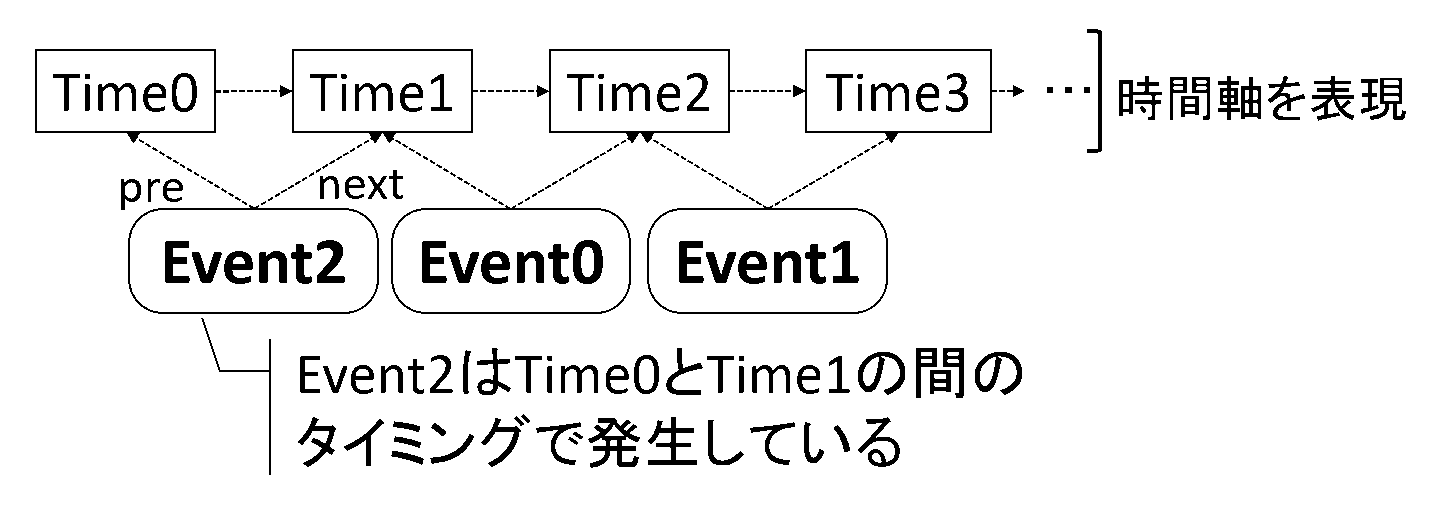
\includegraphics[width=400pt]{./fig/based-model-temporal-logic.eps}
\caption{基礎モデルにおける時間軸とイベントの関係}
\label{fig:based-model-temporal-logic}
\end{figure}

\section{Cookieを包括するモデル}
\label{sec:cookie-model}
\subsection{モデルの特徴}
Ryckらによって提案されたウェブセキュリティモデル\cite{cookie-model}(以下、「Cookieモデル」とする)は、Akhaweらの基礎モデル(\ref{sec:based-model}節参照)を基にCookieの要素を追加したものである。

\subsection{Cookieモデルの能力}
\color{red}
ウェブセキュリティモデルの三要素の一つである「対象のシステムの構造と動作」、及び、「安全性要件」におけるSecurity Invariantsに対してCookieを追加する。
これら以外の要素は基礎モデル\cite{based-model}に準拠する。
\color{black}

\subsection{Cookieモデルにおける時相論理の実装}
基礎モデルでは、時相論理はリクエストやレスポンスといったイベントの発生順序を表現するために用いられている。
Cookieモデルではこれに加えて、対応するリクエストとレスポンス間でのCookieの状態変化を表現するために時相論理を用いている。
Cookieに対しての時相論理はCode\ref{code:cookie-model-temporal-logic}に示すコードで実装される。
\begin{lstlisting}[caption=Cookieに対する時相論理, label=code:cookie-model-temporal-logic]
sig CSState {
	dst: Origin,
	cookies: set Cookie
}

sig CSStateHTTPTransaction extends HTTPTransaction {
	beforeState: CSState,
	afterState: CSState
}{
	beforeState.dst = afterState.dst
	afterState.cookies = beforeState.cookies + (resp.headers & SetCookieHeader).thecookie
	
	beforeState.dst = req.host
}
\end{lstlisting}
このCookieに関する表現は、基礎モデルにおけるCode\ref{code:based-model-httptransaction}を利用している。
1-4行目で定義されているCSStateは、ある時点でのCookieの状態を表現できるクラスである。
また、6-14行目で定義しているCSStateHTTPTransactionは基礎モデルのHTTPTransaction(\ref{sec:based-model-http}節参照)を継承しているクラスであり、既存のクラスに上記のCSStateを付加している。
このCSStateHTTPTransactionにはCSStateを二つ関連付けており、これらはリクエストとレスポンスそれぞれの時点でのブラウザのCookieの状態を表す。
このように記述することで、リクエストとレスポンスのやり取りにおいて起こりうるCookieの変化を11行目のように記述できる。
11行目の具体的な内容は以下のようになる。
\begin{eqnarray*}
& C_{res} = C_{req} + C_{h} &\\
& \left(
\begin{array}{l}
	C_{req} : \mbox{リクエスト時のCookieの集合}\\
	C_{res} : \mbox{レスポンス時のCookieの集合}\\
	C_{h} : \mbox{レスポンスのヘッダに含まれるCookieの集合}
\end{array}
\right) &
\end{eqnarray*}

\begin{figure}[htb]
\centering
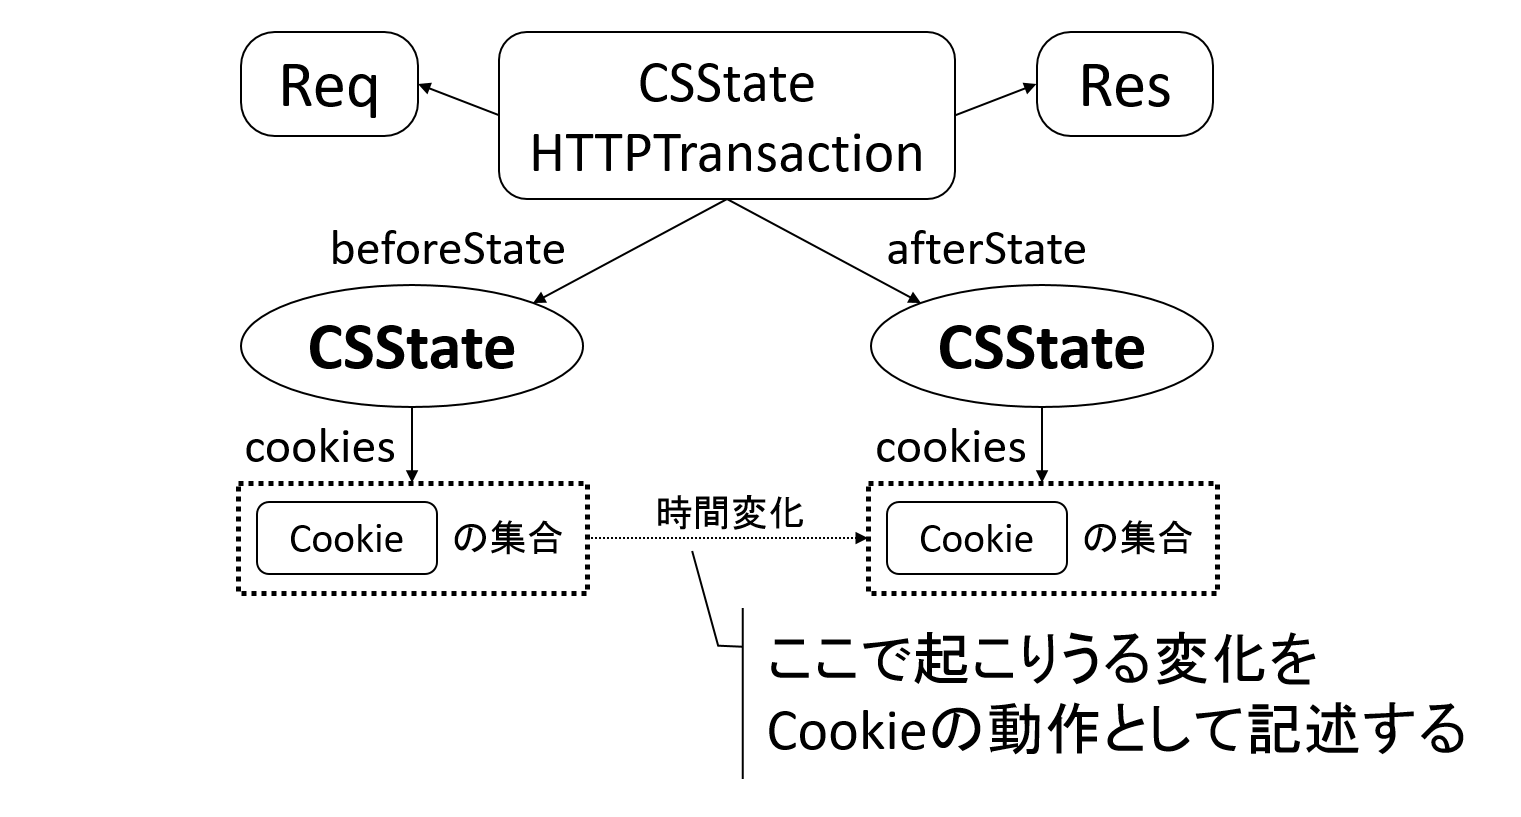
\includegraphics[width=450pt]{./fig/cookie-model-transaction.eps}
\caption{CookieモデルにおけるCookieの時間変化の表現}
\label{fig:cookie-model-transaction}
\end{figure}

\section{既存モデルにおける問題点}
\label{sec:existing-models-problems}
\ref{sec:based-model}、\ref{sec:cookie-model}節の二つの既存モデルの時相論理の表現能力には問題点がある。
それぞれの既存モデルの時相論理の表現能力は以下のようになっている。
\color{red}
\begin{itemize}
\item 基礎モデル \\
リクエストやレスポンスの発生順序を表現するための時間軸を表現できる。
この表現能力はLTLに属する。
\item Cookieモデル \\
対応するリクエストとレスポンス間でのCookieの状態変化を表現できる。
この表現能力はLTLに属する。
\end{itemize}
\color{black}
これらの時相論理の能力では、状態変化はある同一のTransaction間でのみ表現することができ、異なるTransactionにその状態を引き継ぐことはできない。
具体的には図\ref{fig:2transaction-a}のような状況が考えられる。
\begin{figure}[htb]
\centering
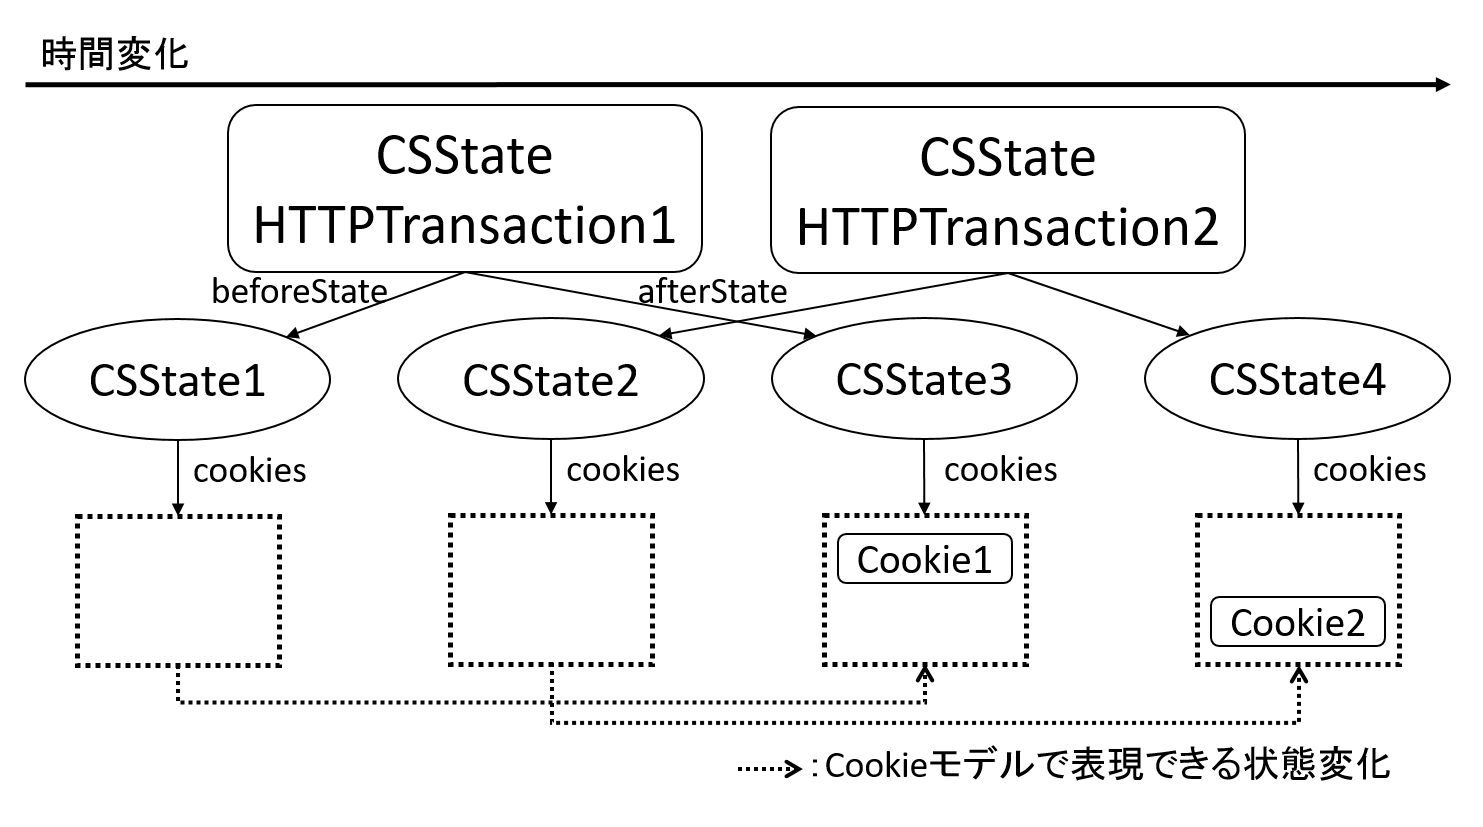
\includegraphics[width=450pt]{./fig/2transaction-a.eps}
\caption{Cookieモデルで表現できる状態変化の一例}
\label{fig:2transaction-a}
\end{figure}
図\ref{fig:2transaction-a}は、ある同一のブラウザからリクエストが二つ連続して送信され、後に送信したリクエストに対するレスポンスが先に行われた状況を表している。
Cookieモデルでの表現能力では、図\ref{fig:2transaction-a}内で示している通りCSState1からCSState3へ、CSState2からCSState4への保有するCookieの集合の変化を表現できる。
しかし、この表現能力ではCSState3で格納されたCookie1がCSState4で格納されていること(図\ref{fig:2transaction-b}のような状態)は起こりえない。
なぜなら、CSState4はCSState3で生じた状態変化を捉えることができないためである。
\begin{figure}[htb]
\centering
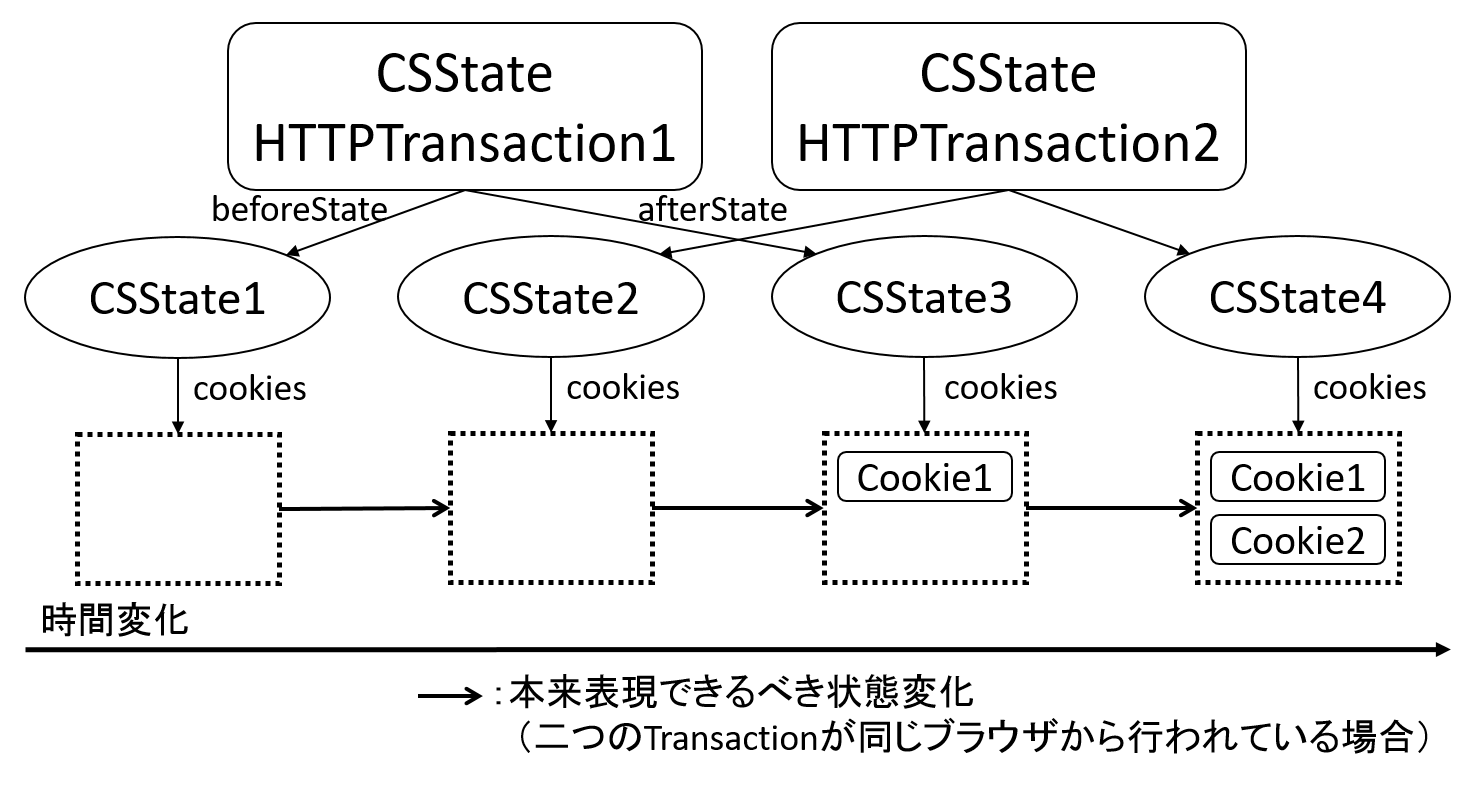
\includegraphics[width=450pt]{./fig/2transaction-b.eps}
\caption{Cookieモデルで表現できない状態変化の一例}
\label{fig:2transaction-b}
\end{figure}
こういった表現できない状態が存在する場合、形式手法で得られた結果に潜在的な危険性が含まれる可能性がある。
したがって、図\ref{fig:2transaction-b}に示すように時間軸に沿った状態変化を捉えられるべきである。
本研究ではこのように時間軸に沿った状態変化をAlloyで実現するための記述法を提案する。
\end{document}
